%!TEX root = ../Main.tex

\section{Loop Generation}
\label{s:LoopGeneration}
After rate inference, our compilation method is as follows:

\begin{enumerate}
\item   Type check and desugar Haskell source code to GHC Core.
\item   A-normalize and eta-expand intermediate code.
\item   \emph{Slurp} out a data flow graph for each series process.
\item   \emph{Schedule} the operators in this graph into an abstract loop nest.
\item   \emph{Concretize} rate variables into loop counters.
\item   \emph{Extract}    new Core code from the loop nest.
\item   Inline library functions into the extracted code.
\item   Complete compilation with GHC's standard pipeline.
\end{enumerate}

A \emph{series process} is a computation that can be expressed as a static, first order, non-recursive data flow graph like that of Figure~\ref{f:nested-contexts}. Data flow graphs are represented by the @Process@ language shown in Figure~\ref{f:Process}. Abstract loop nests are represented by the @Procedure@ language of Figure~\ref{f:Procedure}. In our current implementation stages 1, 7 and 8 are performed by GHC proper using its internal Core language, while stages 2-6 are performed by our GHC plugin. Note that the \emph{Schedule} phase (described in \S\ref{s:SchedulingLoops}) is really the core of our method, with the other phases performing impedance matching between the input and output languages. 


% -----------------------------------------------------------------------------
%!TEX root = ../Main.tex

% -----------------------------------------------------------------------------
\begin{figure}

\begin{tabbing}
MMMM           \= MM \= \kill
$name$  \> $\to$ \> (process name)      \\
$x,~ s$ \> $\to$ \> (value variable)    \\
$a,~ k$ \> $\to$ \> (type variable)
\\[2ex]

$kind$          \> \tt{::=}
                \>      $\tt{*} ~~|~~ \tt{\&}$

\\[2ex]
$type$          \> \tt{::=}
                \>      $a ~~|~~ \tt{Int} ~~|~~ \tt{Float} ~~|~~ ...$ 
\end{tabbing}

\begin{tabbing}
x           \= MM \= MMMMMM \= \kill
$process$ \\
 \> \tt{::=}     
          \> $\tt{process}~~ name~~ (k_{in} : \&)~~ \ov{(a : kind)}$ \\
 \>       \> $~~~~~~~~~~~~~~~~~~~~~~~~~~~~
                        \ov{(x : type)}~~
                        \ov{(s : \tt{Series}~~ k_{in}~~ type)}$      \\
 \>       \> ~~~ $\tt{with}~~     \ov{operator~}~~ 
                \tt{yields}~~       exp$

\\[2ex]
$operator$  \\
 \> \tt{::=}
 \> $\tt{mkSel}
                        ~~ (k_{inner} : \tt{\&})
                        ~~ (x_{sel} : \tt{Sel}~~ k_{outer}~~ k_{inner})$ \\
 \>       \> ~~~ $\tt{from}
                        ~~ k_{outer}
                        ~~ s_{flags}
                        ~~ \tt{in}
                        ~~ \ov{operator}$

 \\[1ex]
 \> $~~|$ \> $s_{out} ~~~~~\tt{<-}
                ~~~ \tt{map}^{\;n}
                        ~~ k_{in}
                        ~~ \ov{type}^{\;n}
                        ~~ exp_{work}
                        ~~ \ov{s_{in}}^{\;n}$ 

 \\[1ex]
 \> $~~|$ \> $s_{out} ~~~~~\tt{<-}
                ~~~ \tt{pack} 
                        ~~ k_{out}
                        ~~ k_{in}
                        ~~ type_{in}
                        ~~ x_{sel}      ~~ s_{in}$

 \\[1ex]
 \> $~~|$ \> $x_{result}~~  
                        \tt{<= fold}~~ k_{in}~~ type_{in}~~ type_{result}~~ s_{in}$ \\
 \>       \> \> $\tt{with}   ~~ exp_{work}
                  ~~    \tt{and}    ~~ exp_{zero}$

 \\[1ex]
 \> $~~|$ \> $x_{vec}~~~~~
                        \tt{<= create}~~ k_{in}~~ type_{in}~~ s_{in}$
\end{tabbing}

\begin{tabbing}
MMMM           \= MM \= \kill
$exp$   
 \> \tt{::=} \>  ... Haskell expressions ...
\end{tabbing} 
\caption{Data Flow Process Description}
\label{f:Process}
\end{figure}



% -----------------------------------------------------------------------------
\begin{figure*}[t]
\begin{center}
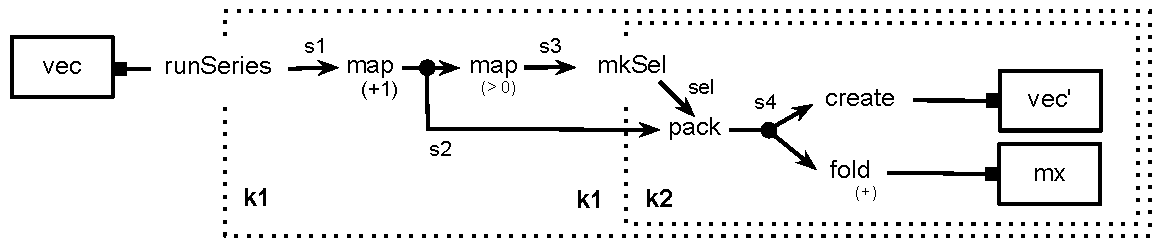
\includegraphics[scale=0.8]{figures/flow-contexts.pdf}
\end{center}
\caption{Nested Rate Contexts for \texttt{filterMax}}
\label{f:nested-contexts}
\end{figure*}


% -----------------------------------------------------------------------------
\subsection{Slurping Processes}
\label{s:Slurping}
The Slurp phase takes a normalized Core module and produces a list of fusible series processes.
\begin{code}
    slurp  :: Module -> [Process]
\end{code}

We supply the Core version of each series process to be fused as a top-level binding in the @Module@. During normalization (stage~2) the application of @runSeries@ that creates the outer-most rate context is also split from the rest of the input code and floated to top-level. The @runSeries@ function itself is implemented in an external Haskell library, and is not part of the Core program given to the loop generator. For our @filterMax@ example, we would then have a binding of the following type:

%
\begin{alltt}
  filterMax_series 
   :: \(\forall\)(k : &). Series k Int -> (Vector Int, Int)
\end{alltt}

This @filterMax_series@ function is the same as @go1@ from Figure~\ref{f:new-filterMax}, after it has been floated to top-level.

The @Process@ language represents the data flow graph for a series process directly, without admitting language features that may be supported by the source language (Haskell) but not representable as a static, first-order data flow graph. If the Core version of the series process cannot be converted to our internal @Process@ language, then the user gets a compile-time warning and the program is compiled via the fallback library discussed in \S\ref{s:Benchmarks}. An example of this is in \S\ref{s:Normalizing}. On the other hand, if we \emph{can} convert the source program to a @Process@, then we guarantee it will be completely fused.


\eject
% -----------------------------------------------------------------------------
The grammar for @Process@ is shown in Figure~\ref{f:Process}, and here is the process description for our @filterMax@ example which encodes the graph in Figure~\ref{f:nested-contexts}:

\begin{code}
process filterMax_s (k1 : &) (s1 : Series k1 Int)
 with { s2 <- map k1 Int (+ 1) s1
      ; s3 <- map k1 Int (> 0) s2
      ; mkSel (k2 : Rate) (sel : Sel k1 k2)
          from  k1 s3  in
        { s4   <- pack   k1 k2 Int sel s2
        ; vec' <= create k2 Int s4
        ; mx   <= fold k2 Int s4 with (+) and 0 } }
 yields (vec', mx)
\end{code}


A $name$ is a process name like @filterMax_s@ (where @_s@ indicates the @Process@ version of this function). We use $x$ and $s$ as (meta) value variables, and by convention use $s$ for series and $x$ for non-series variables. We use $a$ and $k$ as (meta) type variables, where $a$ indicates an element type variable and $k$ indicates a rate.

We use $type$ for element types, with the full set being defined by the host language (Haskell). Our program transformations treat element types abstractly.

A $process$ consists of its name, its type and value parameters, a list of series operators, and an expression that yields the result of the overall process. We have left $exp$ unspecified as this represents expressions from the source language --- Haskell in our case. The rates of all input series must be identical to the first type variable $k_{in}$. This is the rate of the loop that we will generate for this process.

An $operator$ can introduce a new rate context (@mkSel@), be a transformation that converts some series into another one (@map@ and @pack@), or a \emph{sink} that consumes some series and produces a non-series result (@fold@ and @create@). Our operators are explicitly typed, being applied to rate variables that describe the context of each operator, and type arguments that give the element types of each series. Each operator defines a node in the data flow graph, where the binding symbols @<-@ and @<=@ represent the edges. The bindings in an operator list are non-recursive, and variables must be bound before they are used.

The @mkSel@ construct binds the new variables $k_{inner}$ and $x_{sel}$ which are added to the environment of the enclosed list of operators. The @mkSel@ operator itself defines a new rate context $k_{inner}$, inside an outer context $k_{outer}$. It consumes a series of flags $s_{flags}$ and produces a selector $x_{sel}$. In the enclosed operator list, all new series bound at that level must have rate $k_{inner}$. In Figure~\ref{f:nested-contexts} we have drawn @mkSel@ over the dotted line separating the rate contexts @k1@ and @k2@ to indicate that this operator defines the inner context.

The @map@$^{n}$ operator combines several input series $\ov{s_{in}}$ at rate $k_{in}$ using the worker function defined by $exp_{work}$.  The $n$ variable sets the number of input series, though we write just @map@ for @map1@. 

The @pack@ operator takes a series $s_{in}$ of rate $k_{in}$ to a series $s_{out}$ of rate $k_{out}$ using the selector $x_{sel}$. 

The @fold@ operator binds a new variable $x_{result}$ of $type_{result}$ which is the result of reducing the elements of series $s_{in}$ at rate $k_{in}$ using worker function $exp_{work}$ and neutral element defined by $exp_{zero}$. The $type_{in}$ argument is the type of the elements. 

The @create@ operator binds a new variable $x_{vec}$ which is the vector created from elements of the series $s_{in}$, at rate $k_{in}$ and element type $type_{in}$. In Figure~\ref{f:nested-contexts} we have drawn the results produced by @fold@ and @create@ in square boxes to indicate that these are manifest values and not fusible series. 


% -----------------------------------------------------------------------------
\subsubsection{Scoping in Series Process Descriptions}
\label{s:Scoping}
In a process description, the series that are parameters to the process, as well as the new series bound by each operator (to the left of the @<-@ marks) can only be used as series arguments to other operators. These new series are \emph{not in scope} in the worker expressions ($exp_{work}$) and cannot be used in the expression given to @yields@. The results produced by series \emph{sinks} (to the left of the @<=@ marks) are also not in scope of the workers, but can be used in the expression given to @yields@. To put this another way, the workers may refer to environment variables defined outside the process they are contained in, but not variables bound internally in the process. These rules are needed to reject processes like the following:

\begin{code}
  process badNorm (k1 : &) (s1 : Series k1 Float)
   with { total <= fold k1 Float s1 with (+) and 0
        ; s2    <- map  k1 Int  (/ total) s1
        ; vec   <= create k1 Int s2 }
   yields vec
\end{code}

Here, because the worker function for @map@ refers to the result @total@, to evaluate this code we would need to finish computation of the @fold@ operator before embarking on the @map@. However, as we will see in \S\ref{s:SchedulingLoops}, we intend to compile each process description into a single fused loop, and this is not possible for @badNorm@. It would be possible to automatically split such \emph{compound} processes into individual parts before passing them to the scheduler defined in \S\ref{s:SchedulingLoops}, but we leave this to future work.


% -----------------------------------------------------------------------------
\subsubsection{Normalizing the Input Core Program }
\label{s:Normalizing}
The Core version of a series process is easy to slurp to the @Process@ language of Figure~\ref{f:Process}, provided we make use of the explicit type annotations in Core, and perform some appropriate normalizations beforehand.

Before conversion, we a-normalize and eta-expand the definitions in the module so that every intermediate series has an explicit name. These names are identified with the edges of the extracted data-flow graph. We also use a preparation transform to force worker functions to be floated into their use sites --- so that combinators like @mkSel@, @map@ and @fold@ are directly applied to workers. For example, as part of the @filterMax@ example we get the following Core snippet:
%
\begin{alltt}
  mkSel @k1 @(Vector Int, Int) s1
    (\(\Lambda\)(k2 : &). \(\lambda\)(sel : Sel k1 k2). 
     let s4 : Series k2 Int
            = pack @k1 @k2 @Int sel s2
     in ...)
\end{alltt}

With the above code we already have all the information we need to produce the equivalent snippet of the @Process@ language:
%
\begin{alltt}
  mkSel (k2 : &) (sel : Sel k1 k2) 
       from k1 s1 in 
    \{ s4  <= pack k1 k2 Int sel s2
      ... \}
\end{alltt}

Although the example above is really just a change of syntax, as mentioned in \S\ref{s:Slurping} the real point is that the @Process@ language is smaller than the input Core language. We use the intermediate @Process@ language primarily as way to reject features of the input language that cannot be expressed as static, first order, non recursive data flow graphs. For example, the following function cannot be converted to a @Process@ because we have no way to represent the inner @if@ construct. 

\begin{alltt}
 badSwitchy :: \(\forall\)(k : &). Bool 
            -> Series k Int -> Series k Int -> Int
 badSwitchy flag s1 s2
  = fold (+) 0 (if flag then (map (* 2) s1) 
                        else (map (* 4) s2)
\end{alltt}

The above function does not express a \emph{static} data flow graph, because we do not statically know which input series to use for the @fold@ operator. We have no way to compile this function into a single loop that fuses the contained @fold@ and @map@ operators, even though they operate on series all at the same rate. 


% -----------------------------------------------------------------------------
\subsubsection{Processes are Hyper-strict}
A process description is naturally hyper-strict, meaning every value that is mentioned will be computed. If we are not careful then this can lead to unused values being computed. For example, consider the following function that choses between two fold results:

\begin{alltt}
strictSwitchy :: \(\forall\)(k : &). Bool 
              -> Series k Int -> Series k Int -> Int
strictSwitchy flag s1 s2
 = choose flag (fold (+) 0 (map (* 2) s1))
               (fold (+) 0 (map (* 4) s2))
\end{alltt}

The above function is similar to @badSwitchy@ from the previous section, except that we have used the @if@-like function @choose@ to select between the two folded results. When evaluated using Haskell semantics, the fact that @choose@ is non-strict in both arguments will mean that only one of the @fold@ results will be computed. However, a-normalizing and then slurping a @Process@ from this code produces:

\begin{alltt}
 process strictSwitchy (k : &) (flag : Bool) 
          (s1 : Series k Int) (s2 : Series k Int)
  with \{ s3 <- map  k Int (* 2) s1
       ; s4 <- map  k Int (* 4) s2
       ; x1 <= fold k Int s3 with (+) and 0
       ; x2 <= fold k Int s4 with (+) and 0 \}
  yields (choose flag x1 x2)
\end{alltt}

As mentioned earlier, we intend to compile this whole process description into a single loop. If we use the code above then both reductions will be computed at the same time, before choosing the desired result after the loop completes. 

To avoid this problem automatically we could check whether values produced with @fold@ or @create@ are used strictly in the expression given to @yields@, and if not, emit a warning to the user. It may also be possible to automatically massage the source program or @Process@ descriptions to ensure that unused results are not computed, but we have not investigated this further. As mentioned in \S\ref{s:Introduction}, a primary client of our new fusion system is Data Parallel Haskell (DPH), and the DPH vectorizer eliminates conditional operators like @choose@ as part of its existing vectorization process. 

%!TEX root = ../Main.tex

% -----------------------------------------------------------------------------
\begin{figure}
\begin{tabbing}
MMMMx           \= MM \= \kill
$name$  \> $\to$ \> (procedure name)            \\
$x,~ s$ \> $\to$ \> (value variable)            \\
$a,~ k$ \> $\to$ \> (type variable)             
\\[1ex]

$vec$   \> $\to$ \> (vector variable)           \\
$acc$   \> $\to$ \> (accumulator)
\\[2ex]

$kind$          \> \tt{::=}
                \>      $\tt{*} ~~|~~ \tt{\&}$

\\[1ex]
$type$          \> \tt{::=}
                \>      $a ~~|~~ \tt{Int} ~~|~~ \tt{Float} ~~|~~ ...$ 
\end{tabbing}

\begin{tabbing}
MMMMx           \= MM \= M \= MMMM \= \kill
$procedure$ 
 \> \tt{::=}    
        \> $\tt{procedure}~ name~ (k_{in} : \&)~ \ov{(a : kind)}$ \\
 \>     \> ~~~~~~~~~~~~~~~~~~~~~~~~~~~~ $\ov{(x : type)} 
                ~~ \ov{(s : \tt{Series}~ k_{in}~ type)}$     \\
 \>     \> ~~~$\tt{with}~~ \ov{nest}
                ~~ \tt{yields}~~ exp$
\end{tabbing}

\begin{tabbing}
MMMMx            \= MM \= x \= MMMM \= \kill
$nest$ 
 \> \tt{::=}       \> $\tt{loop}~~ k$            \\
 \>             \> \> \tt{start}  \> $\ov{stmtstart}$   \\
 \>             \> \> \tt{body}   \> $\ov{stmtbody}$    \\
 \>             \> \> \tt{inner}  \> $\ov{nest}$        \\
 \>             \> \> \tt{end}    \> $\ov{stmtend}$     
 \\[1ex]

 \> $~~|~~$     \> $\tt{guard}~~ (k_{inner} : \&)~~   
                        \tt{with}~~ k_{outer}~~ x_{flag}$ \\
 \>             \> \> \tt{body}   \> $\ov{stmtbody}$      \\
 \>             \> \> \tt{inner}  \> $\ov{stmtend}$
\end{tabbing}

\begin{tabbing}
MMMMx            \= Mx \= MMMx \= MMMM \= \kill
$stmtstart$     
 \> \tt{::=}    \> ~~ $vec$      \> $\tt{ =}~~~ \tt{newVec}~~ k$         \\[0.5ex]
 \> $~~~|$      \> ~~ $acc$      \> $\tt{ =}~~~ \tt{newAcc}~~ exp_{zero}$
\\[1.5ex]

$stmtbody$      
 \> \tt{::=}    \> ~~ $x_{elem}$ \> $\tt{ =}~~~ x'_{elem}$               \\[0.5ex]
 \> $~~~|$      \> ~~ $x_{elem}$ \> $\tt{ =}~~~ \tt{next}~~ k~~ s_{in}$  \\[0.5ex]
 \> $~~~|$      \> ~~ $x_{elem}$ \> $\tt{ =}~~~ exp_{worker}~~ \ov{x_{elem}} $  \\[0.5ex]
 \> $~~~|$      \> ~~ $acc$      \> $\tt{:=}~~~ exp_{worker}~~ acc~~ x_{elem}$  \\[0.5ex]
 \> $~~~|$      \> ~~ $\tt{writeVec}~~ k~~ vec~~ x_{elem}$
\\[1.5ex]

$stmtend$
 \> \tt{::=}    \> ~~ $x_{result}$ \> $\tt{ =}~~~ \tt{read}~~ acc$      \\[0.5ex]
 \> $~~~|$      \> ~~ $\tt{sliceVec}~~ k~~ vec$
\end{tabbing}

\caption{Series Procedures as Abstract Loop Nests}
\label{f:Procedure}
\end{figure}


%!TEX root = ../Main.tex

% -----------------------------------------------------------------------------
\begin{figure*}[ht]
\fbox{$process \Rightarrow procedure$}
$$
\infer  { \begin{aligned}
           & \tt{process}~~~~
                ~~ name
                ~~      (k_{in} : \tt{\&})
                ~~      \ov{(a : kind)}
                ~~      \ov{(x : type)}
                ~~      \ov{(s_{n} : \tt{Series}~ k_{in}~ type_n)}^{n}
                ~~ \tt{with}
                ~~      \ov{operator}
                ~~ \tt{yields}
                ~~      exp
          \\ 
          \Rightarrow~~
          & \tt{procedure}
                ~~ name
                ~~      (k_{in} : \tt{\&})
                ~~      \ov{(a : kind)}
                ~~      \ov{(x : type)}
                ~~      \ov{(s_{n} : \tt{Series}~ k_{in}~ type_n)}^{n}
                ~~ \tt{with}
                ~~      nest
                ~~~~~~~~~~ \tt{yields}
                ~~      exp
          \end{aligned}
        }
        { \tt{loop}~~ k_{in}~~
                \tt{body}~~ \{ \ov{s^{elem}_n ~\tt{=}~ \tt{next}~~ k_{in}~~ s_{n}}^{n} \}
        ~~ \vdash
        ~~      \ov{operator}
        ~~ \Rightarrow
        ~~      nest
        }
$$

\medskip
\fbox{$nest \vdash \ov{operator} \Rightarrow nest$}
$$
\infer  {  nest  
        ~~ \vdash
                ~~ \tt{mkSel}
                ~~      (k_{inner} : \tt{\&})
                ~~      (x_{sel} : \tt{Sel}~~ k_{outer}~~ k_{inner})
                ~~ \tt{from}
                ~~      k_{outer}
                ~~      s_{flags}
                ~~ \tt{in}
                ~~ \ov{operator}
        ~~ \Rightarrow
                ~~ nest'
        }
        { nest 
        ~~ \rhd
        ~~ (k_{outer}~ \times
                ~~ \tt{inner}
                ~~ \{   ~~ \tt{guard}~~ (k_{inner}~ : \tt{\&})
                        ~~ \tt{with}~~ k_{outer}~~ s^{elem}_{flags} 
                ~~ \})
        ~~ \vdash
        ~~      \ov{operator}
        ~~ \Rightarrow
        ~~      nest'
        }
$$


\begin{tabbing}
MMMM \= MMMM \= MMMMMMMMMMMMMMMMMMMM \= Mx \= MM \= MMMx \= \kill

% -- map ----------------
 \> $nest~ \vdash$    
        \> $s_{out} ~~~~~\tt{<-}
                ~~~ \tt{map}^{\;n}
                        ~~ k_{in}
                        ~~ \ov{type}^{\;n}
                        ~~ exp_{work}
                        ~~ \ov{s_{in}}^{\;n}$

\> $\Rightarrow$ 
        \> $nest$
        \> $\rhd~~ (k_{in}$
        \> $\times~~ \tt{body}~~~~ 
                \{~~ s^{elem}_{out} ~~~~~~\tt{=}~~ exp_{work}~~ \ov{s^{elem}_{in}}^{\;n} \} )$ 
\\[1em]


% -- pack --------------
 \> $nest~ \vdash$
        \> $s_{out} ~~~~~\tt{<-}
               ~~~ \tt{pack} 
                       ~~ k_{out}
                       ~~ k_{in}
                       ~~ type_{in}
                       ~~ x_{sel}
                       ~~ s_{in}$
\> $\Rightarrow$
        \> $nest$
        \> $\rhd~~ (k_{out}$
        \> $\times~~ \tt{body}~~~~ 
                \{~~ s^{elem}_{out} ~~~~~~\tt{=}~~ s^{elem}_{in} ~~\})$
\\[1em]


% -- fold --------------
 \> $nest~ \vdash$
        \> $x_{result}~~  
                        \tt{<= fold}~~ k_{in}~~ type_{in}~~ type_{result}~~ s_{in}$ 
 \> $\Rightarrow$
        \> $nest$
        \> $\rhd~~ (\top$
        \> $\times~~ \tt{start}~~   
                \{~~ x^{acc}_{result} ~~~~\tt{=}~~ \tt{newAcc}~~ exp_{zero} ~~\})$
 \\[0.5ex]     


 \>     \> \hspace{5em} $\tt{with}   ~~ exp_{work}
                      ~~ \tt{and}    ~~ exp_{zero}$
 \>     \> 
        \> $\rhd~~ (k_{in}$
        \> $\times~~ \tt{body}~~~~    
                \{~~ x^{acc}_{result}~~ \tt{:=}~~ exp_{work}~~ x^{acc}_{result}~~ s^{elem}_{in} ~~\})$
 \\[0.5ex]


 \>     \>
 \>     \> 
        \> $\rhd~~ (\top$
        \> $\times~~ \tt{end}~~~~~~ 
                \{~~ x_{result}~~~~~ \tt{=}~~ \tt{read}~~ x^{acc}_{result} ~~\})$
 \\[1em]


% -- create ------------
 \> $nest~ \vdash$    
        \> $x_{vec}~~~~~
                        \tt{<= create}~~ k_{in}~~ type_{in}~~ s_{in}$
 \> $\Rightarrow$
        \> $nest$
        \> $\rhd~~ (\top$
        \> $\times~~ \tt{start}~~
                \{~~ x_{vec}~~~~~~~~ \tt{=}~~ \tt{newVec}~~ k_{in} ~~\})$
 \\[0.5ex]

 \>     \>
 \>     \> 
        \> $\rhd~~ (k_{in}$
        \> $\times~~ \tt{body}~~~~
                \{~~ \tt{writeVec}~~ k_{in}~~ x_{vec}~~ s^{elem}_{in}~~ \})$
 \\[0.5ex]

 \>     \>
 \>     \>
        \> $\rhd~~ (\top$
        \> $\times~~ \tt{end}~~~~~~
                \{~~ \tt{sliceVec}~~ k_{in}~~ x_{vec}~~ \})$
\end{tabbing}
\caption{Scheduling Series Processes into Procedures}
\label{f:Scheduling}
\end{figure*}



% -----------------------------------------------------------------------------
\subsection{Scheduling Processes into Procedures}
\label{s:SchedulingLoops}
The Schedule phase takes a list of processes and converts it to a list of procedures.
%
\begin{code}
  schedule    :: [Process] -> [Procedure]
\end{code}

The definition of @Procedure@ is given in Figure~\ref{f:Procedure}. A @Procedure@ expresses the same computation as a @Process@, except that it is defined by an abstract, imperative loop nest instead of an operator graph. In Figure~\ref{f:Procedure} the fields of the @loop@ construct represent the \emph{anatomy} of the loop, similarly to \cite{Shivers:anatomy-of-a-loop}. The idea of representing a loop in this ``broken up'' format also appears in work by Waters on series expressions \cite{Waters:series-expressions, Waters:series-expressions-interpretation}, which was inspired by the @loop@ macro package of Common LISP~\cite{Steele:lisp}. 

For example, here is a simple @Process@ that sums the elements of an input series @s1@:
%
\begin{code}
 process sum_s (k : &) (s1 : Series k Int)
  with { x1 <= fold k Int s1 with (+) and 0 }
  yields x1
\end{code}


\eject
% ----------------------------------------------------------------------------
\noindent
The scheduled procedure is then:
%
\begin{code}
 procedure sum_d (k : &) (s1 : Series k Int) 
  with loop k
       start { x1_acc   = newAcc 0 }
       body  { s1_elem  = next k s1
             ; x1_acc  := (+) x1_acc s1_elem }
       inner {}
       end   { x1       = read x1_acc }
  yields x1
\end{code}

The @start@ field of a @loop@ holds setup statements to execute before entering the loop proper; @body@ contains the statements to execute for each iteration; @inner@ holds some inner nests to run for every iteration, and @end@ contains cleanup code that runs after the loop has completed. In future we elide empty fields, instead of writing @inner {}@ and so on.

In the @sum_d@ example, @x1_acc = newAcc 0@ creates a new accumulator @x1_acc@. The statement @s1_elem = next k s1@ takes the next element from @s1@. The statement @x1 = read x1_acc@ reads the accumulator. Note that the @next@, update @(:=)@ and @read@ statements are side effecting, imperative operations. 

Now, suppose we wanted a procedure like @sum_d@ that also computed the product of @s1@ concurrently with its sum, then added both results together. We would do this by appending an extra statement to each of the fields of the nest, and changing the yielded expression.

\begin{code}
procedure sumProd (k : &) (s1 : Series k Int)
 with loop k
      start { acc1      = newAcc 0
            ; acc2      = newAcc 1 }          *NEW
      body  { s1_elem   = next k s1
            ; acc1     := (+) acc1 s1_elem
            ; acc2     := (*) acc2 s1_elem }  *NEW
      end   { x1        = read acc1
            ; x2        = read acc2 }         *NEW
 yields (x1 + x2)                         *CHANGED
\end{code}

In general terms, to convert a process into a procedure we consider each operator from the process in turn, and insert statements into the procedure that implement that operator. The fact that our procedure is expressed as an \emph{anatomy} of separate @start@, @body@ and @end@ fields means that we can produce code that interleaves the computation of each operator. This interleaving of code is the primary mechanism which lets us deal with branching data flows, which we will return to in \S\ref{s:Related}. 

The scheduling process is formalized in Figure~\ref{f:Scheduling}, and we will give more examples in coming sections. The top level judgment $process \Rightarrow procedure$ converts a process into a similarly named procedure. Note that the resulting procedure has the same parameters and yielded expression, but its implementation has changed from an operator list into an abstract loop nest.

The $\rhd$ operator used in Figure~\ref{f:Scheduling} has the following type:
%
\[ \rhd : nest \to ((rate + \top) \times field) \to nest \]
%
where $field$ is one of the fields attached to the @loop@ or @guard@ constructs of Figure~\ref{f:Procedure} (@start@, @body@ and so on). The application ($n \rhd k \times f$) recursively descends into the nest $n$ until it finds the @loop@ or @guard@ construct that matches rate $k$, and then appends the statements in field $f$ to the similar field of that construct. When searching for matching rates we use the $k$ in (@loop@ $k$) and the $k_{inner}$ in ($\tt{guard}~ (k_{inner} : \&)~~ \tt{with}~~ ...$ ). The @guard@ construct is an abstract @if@ expression, and $k_{inner}$ corresponds to the number of times the body is entered. In some rules we use $\top$ in place of a real rate variable, which matches the rate of the outer-most loop construct in the nest.


% -----------------------------------------------------------------------------
\subsubsection{Scheduling Maps}
\label{s:SchedulingMaps}
As an example of how to schedule the @map@ operator, suppose we have a process like @sumProd@ from \S\ref{s:SchedulingLoops} that also performs a @map fn@ on the elements before taking the sum and product, for some arbitrary @fn@. Here is the full process description:

\begin{code}
 process sumProdFn (k : &) (s1 : Series k Int)
  with { s2  <- map  k Int fn s1
       ; xs  <= fold k Int s2 with (+) and 0
       ; xp  <= fold k Int s2 with (*) and 1 }
  yields (xs + xp)
\end{code}
%
Using just the first rule in Figure~\ref{f:Scheduling} and the one for @map@ would produce the following procedure, where we still need to schedule the two @fold@ operators:
%
\begin{code}
 procedure sumProdFn (k : &) (s1 : Series k Int)
  with loop k
       body  { s1_elem   = next k s1
             ; s2_elem   = fn s1_elem }
  yields (xs + xp)                  ** NOT FINISHED
\end{code}
%
Importantly, note that the intermediate variables @s1_elem@ and @s2_elem@ are named after the corresponding series @s1@ and @s2@. In Figure~\ref{f:Scheduling} this naming convention is indicated by the superscript on variable names, so $s^{elem}$ is a concrete variable name related to the name $s$. We use this trick to avoid maintaining an environment that maps series names ($s$) to the variable names that bind their individual elements ($s_{elem}$). We similarly relate the names of non-series variables ($x$) to their corresponding accumulators ($x^{acc}$). 

Returning to Figure~\ref{f:Scheduling}, the rule for @fold@ adds statements to the nest that first initialize an accumulator, update it in the body of the loop, and then read back the final value. The accumulator lives for the entirety of the loop, so we insert the statements to initialize and read its value in the outer most context, indicated by $\top$.

\eject
Scheduling the two fold operations of @sumProdFn@ produces the following.

\begin{code}
 procedure sumProdFn (k : &) (s1 : Series k Int)
 with loop k
      start { xs_acc    = newAcc 0             *NEW
            ; xp_acc    = newAcc 1 }           *NEW
      body  { s1_elem   = next k s1
            ; s2_elem   = fn s1_elem   
            ; xs_acc   := (+) xs_acc s2_elem   *NEW
            ; xp_acc   := (*) xp_acc s2_elem } *NEW
      end   { xs        = read xs_acc          *NEW
            ; xp        = read xp_acc }        *NEW
 yields (xs + xp)
\end{code}

When we convert this back to concrete Core code in the next section, we will generate the outer structure of the loop that causes the statements in the body to be evaluated the correct number of times This is governed by the associated rate variable @k@. 


% -----------------------------------------------------------------------------
\subsubsection{Scheduling Pack and Create}
\label{s:SchedulingPacks}
Operators from @mkSel@ contexts in the process description are scheduled into the body of an abstract @if@ statement represented by the @guard@ construct of Figure~\ref{f:Procedure}. A @guard@ binds the rate variable $k_{inner}$ for the inner context, and is also tagged with the rate $k_{outer}$ of the outer context. With @guard@, the @body@ and @inner@ fields contain more statements to run when the corresponding flag $x_{flag}$ is true. The @inner@ nest is needed when a packed series is packed again using a different selector, as this creates a more deeply nested parallel context. The NestedFilter example described in \S\ref{s:Benchmarks} does this.

Figure~\ref{f:filterMax-nest} shows the procedure generated for the explicitly typed version of @filterMax@ back in Figure~\ref{f:new-filterMax}, whose process description is in \S\ref{s:Slurping}. On the right of each statement we show the series operator that statement is associated with. 

Scheduling the use of @create@ has added three separate statements to the nest: one to allocate the new vector buffer; one to write elements into it, and one to destructively slice it down to the final size by overwriting its length field. Note that the use of the $\rhd$ operator in the corresponding rule from Figure~\ref{f:Scheduling} ensures that the result vector is only written to inside the body of the @guard@. Also, note that @newVec@ and @sliceVec@ statements are tagged with @k2@, which is not in scope in the outer context. This reflects that fact that the length of the result vector cannot be known until the loop completes, as only then will we know how many times the body of the @guard@ was entered. We will fix this in the \emph{concretization} phase described in the next section, by rewriting the code to keep track of the length of the result vector.

Interestingly, the @pack@ operation becomes a trivial renaming, as shown in the first statement of the inner @body@ field of Figure~\ref{f:filterMax-nest}. Recall that in the version of @filterMax@ from Figure~\ref{f:new-filterMax}, the pack operation was written @s4 = pack k1 k2 Int sel s2@, and here we have scheduled it as just @s4_elem = s2_elem@. It is the @mkSel@ function that actually creates the selector context, and that context is expressed here as a @guard@ construct. When looking at the source code of @filterMax@, we might imagine that pack would perform some sort of indexing operation, after the discussion in \S\ref{s:SelectorsAndPacking}. However, when the code is expressed in the form of Figure~\ref{f:filterMax-nest} the current index into each series is implicit. 

From a logical / type-theory perspective we view @pack@ as a \emph{coercion} from a series of the outer rate (@k1@) to a series of the inner rate (@k2@). This coercion is justified by \emph{evidence} that these rates are related, which is expressed as our selector @sel@. However, our compilation process eliminates the selector completely, so the physical packing operation as described in \S\ref{s:SelectorsAndPacking} is never performed.


\begin{figure}
\begin{code}
procedure filterMax_d (k1 : &) (s1 : Series k1 Int)
with loop k1
 start { vec'     = newVec k2             *create
       ; mx_acc   = newAcc 0       }      *fold max
 body  { s1_elem  = next k1 s1
       ; s2_elem  = (+ 1) s1_elem         *map (+ 1)
       ; s3_elem  = (> 0) s2_elem  }      *map (> 0)
 inner guard (k2 : &) with k1 s3_elem
       body { s4_elem = s2_elem           *pack
            ; writeVec k2 vec' s4_elem    *create
            ; mx_acc := max mx_acc s4_elem} *fold max
 end   { sliceVec k2 vec'                 *create
       ; mx       = read mx_acc }         *fold max
yields (vec', mx)
\end{code}
\caption{Procedure for \texttt{filterMax}}
\label{f:filterMax-nest}
\end{figure}


% -----------------------------------------------------------------------------
\subsection{Concretization}
\label{s:Concretization}
The concretization phase rewrites constructs that use type level rate variables into ones that use real indices and loop counters. 
\begin{code}
  concretize :: [Procedure] -> [ProcedureI]
\end{code}

The @ProcedureI@ language is very similar to @Procedure@ in Figure~\ref{f:Procedure} except that every appearance of a rate variable in @Procedure@ is replaced by loop counter or known length in @ProcedureI@.\footnote{In our real implementation we use the same data type to represent both, and simply fill-in accumulation variables during concretization.} The concrete version of @filterMax@ is shown in Figure~\ref{f:filterMax-concrete}, which is the transformed version of Figure~\ref{f:filterMax-nest}. 

Deciding whether to change a rate variable to a loop counter (like @k1@ to @k1_ix@), accumulator (@k2@ to @k2_acc@) or a known length (@k1@ to @length s1@) is based on the form of the construct being rewritten. For example, for @sliceVec@ we always rewrite its rate variable to a similarly named accumulator.

The operator @guard (k2 : &) with k1 s3_elem@ in Figure~\ref{f:filterMax-nest} changes to @guardI (k2_ix: Int) k2_acc with s3_elem@ in Figure~\ref{f:filterMax-concrete}. For each @guard@ we also insert an accumulator (@k2_acc@) to keep track of how many times the guard is entered. The new @guardI@ construct executes by first checking the flag @s3_elem@, and if it is true, reads @k2_acc@ to get the current entry counter and binds it to @k2_ix@ before evaluating the body. In the application of @writeVecI@ this index @k2_ix@ is then used when constructing the filtered result vector @vec'@. The final @sliceVec@ statement is also rewritten to use @k2_acc@, so it knows the final length.

The last task is to rewrite rate variables on @loop@ constructs and @newVec@ statements to use the lengths of known series. For this we simply look in the environment for a series whose type contains the same rate variable and use its length. If there are multiple series with the same rate variable then we just choose the first one --- as all series tagged with the same rate are guaranteed to have the same length. 


% -----------------------------------------------------------------------------
\begin{figure}
\begin{code}
procedure filterMax_c (k1 : &) (s1 : Series k1 Int)
with loopI (k1_ix : Int) (length s1)
 start { vec'     = newVecI (length s1)    *CHANGED
       ; acc      = newAcc  0 
       ; k2_acc   = newAcc  0 }            *NEW
 body  { s1_elem  = nextI k1_ix s1         *CHANGED
       ; s2_elem  = (+ 1) s1_elem
       ; s3_elem  = (> 0) s2_elem  }
 inner guardI (k2_ix : Int) k2_acc with s3_elem            
                                           *CHANGED
       body { s4_elem = s2_elem
            ; writeVecI k2_ix vec' s4_elem *CHANGED
            ; acc    := max acc s4_elem }
 end   { sliceVecI k2_acc vec'             *CHANGED
       ; mx       = read acc }            
yields (vec', mx)
\end{code}
\caption{Concrete Procedure for \texttt{filterMax}}
\label{f:filterMax-concrete}
\end{figure}


% -----------------------------------------------------------------------------
\subsection{Extracting Implementation Code}
\label{s:Extract}
The Extract phase takes our concretized list of procedures and converts them back to a module of imperative flavoured Core code. We end up with a top-level binding for each @Procedure@, which mirrors the @slurp@ phase from \S\ref{s:Slurping}.
%
\begin{code}
  extract     :: [Procedure] -> Module
\end{code}
%
The extracted code for @filterMax@ is shown in Figure~\ref{f:filterMax-extracted}. As we can see, this final phase is again mostly a change of syntax. The real work of fusion has been performed by the scheduling phase, and the concretization pass in the previous section has already reduced the abstraction level of our program to something that looks like real loop code. 

In the extracted code the @loopI@ and @guardI@ constructs have changed to calls to similarly named functions. As we will see in the next section, these can be implemented as Haskell library functions and then inlined, or transformed to into tail recursive loops as discussed in \S\ref{s:LoopWinding}.


% -----------------------------------------------------------------------------
\begin{figure}
\begin{alltt}
filterMax_x :: \(\forall\)(k1 : &)
            .  Series k1 Int -> (Vector Int, Int)
 = \(\Lambda\)(k1 : &).
   \(\lambda\)(s1 : Series k1 Int).
   let vec'   : Vector Int = newVec @Int (length s1)
   let acc    : Ref Int    = newRef @Int 0    
   let k2_acc : Ref Int    = newRef @Int 0    
   let _ : Unit
       = loopI (length s1)
         (\(\lambda\)(k1_ix : Int).
          let s1_elem = next @k1 @Int s1 k1_ix 
          let s2_elem = add  @Int 1    s1_elem 
          let s3_elem = gt   @Int 0    s2_elem 
          let _  : Unit
              = guardI k2_acc s3_elem
                 (\(\lambda\)(k2_ix : Int).
                  let s4_elem = s2_elem
                  let _ = writeVec @Int
                            vec k2_ix s4_elem 
                  let _ = writeRef @Int acc
                            (max (readRef @Int acc) 
                                 s4_elem) 
                  in ()) 
          in ()) 
   let k2_ix : Int        = readRef  @Int k2_acc
   let vec'' : Vector Int = sliceVec @Int k2_ix vec'
   let mx    : Int        = readRef  @Int acc
   in  (vec'', mx)
\end{alltt}
\caption{Extracted Imperative Core Code for \texttt{filterMax}}
\label{f:filterMax-extracted}
\end{figure}

